% 张量
% 张力|函数|线性函数|双线性函数|矩阵运算|张量|向量|映射|矩阵

\pentry{矩阵\upref{Mat}}

% 未完成: 线性映射词条需要从抽象角度重新创作;线性映射词条大概率会引用映射词条,到时候要在预备知识中删除映射词条这一项
% 补充: 应该还需要矩阵作为预备知识, 而矩阵会需要线性映射作为预备

“张量”一词最早出现在结构力学里,用来描述应力的性质,因此被叫做\textbf{张力(tensor)},这个名字沿用到了今天,只是翻译改成了\textbf{张量}.现在我们知道,张力只是一种更一般的数学对象,张量,的特例,而这种对象在物理学的各个角落频繁出现.因此,我们会从现代角度,从根本上定义张量的概念,并展示如何将张量表示成常见的多维矩阵的形式.

本词条性质更接近于循序渐进的课本,而非罗列概念定理的词条,请留意.为了便于理解本条内容,读者应有扎实的线性代数功底.

本词条所介绍的是最根本的张量的定义,没有附加任何其它结构或限制,也暂未使用爱因斯坦求和约定,以方便初学者入门.对于张量的协变和逆变等概念,请参考本章本词条之后的内容.

\subsection{简介}

张量本身,是一种多重线性映射.特别地,二阶张量可以看成是把两个向量映射成一个数字,也可以看成是把一个向量映射成一个向量.这里的数字是在定义以上向量的域中的,在物理中一般是实数域或复数域.

许多物理量都可以看成是线性映射.比如说,质量可以看成一个张量,它把加速度向量映射成一个力向量;转动惯量也可以看成一个张量,它把角速度向量映射成一个角动量向量.张量的阶数不同,性质看起来也不同,但它们都有一个共性,即满足线性性质.在未来的学习中遇到张量时,不妨思考“这个张量是为了把什么映射为什么而定义的”,有利于加深理解.

\subsection{$1$-线性函数,$2$-线性函数以及它们的表示}

我们知道,给定两个向量空间$V$和$W$,我们可以构造从$V$到$W$的线性映射.在这种情况下,自变量只有一项,因变量也只有一项.多重线性映射,比如$k$重线性映射,就是拿一系列$V_1, V_2, \cdots, V_k$来进行一个多元映射,让这个多元映射中的某一个自变量$\bvec{v}_i\in V$单独变化时,映射看起来就像一个普通的线性映射.

最简单的情况,就是考虑$W$是一个一维空间.在这种情况下,$W$也可以看作实数域本身,而不是线性空间.将集合中的元素映射到数字集合上的映射,我们用一个特殊的术语来称呼,\textbf{函数},也就是中学课程中函数一词,毕竟中学所涉及到的映射基本上都是实数到实数的映射,自然被称为函数.那么当线性映射的目标是一维的$W$时,由于此时$W$被看成实数域,我们特别地把这个映射称为\textbf{线性函数}.下面,我们就要用线性函数的概念来一步步引入多重线性映射和张量的概念及其表示.

\subsubsection{线性函数用向量表示}
\begin{definition}{线性函数}
给定实数域$\mathbb{R}$上的$n$维线性空间$V$,称$f:V\rightarrow \mathbb{R}$为$V$到域$\mathbb{R}$上的一个\textbf{线性函数},如果$f$满足以下线性性:对于任意的$\bvec{v}_1, \bvec{v}_2\in V$和$a_1, a_2\in\mathbb{R}$,都有$a_1f(\bvec{v}_1)+a_2f(\bvec{v}_2)=f(a_1\bvec{v}_1+a_2\bvec{v}_2)$.
\end{definition}

如果把域$\mathbb{R}$本身看成一个一维的线性空间,那么线性函数就是$V$到这个一维空间上的线性映射.因此,我们只需要任取一个$V$的基,研究基向量被$f$映射到哪里,就可以计算出任意的$\bvec{v}\in V$被映射到哪里了.

设$V$有基$\{\bvec{e}_i\}_{i=1}^n$.如果基向量$\bvec{e}_i$被映射为$f(\bvec{e}_i)=m_i\in\mathbb{R}$,那么对于任意的向量$\bvec{v}=a_1\bvec{e}_1+a_2\bvec{e}_2+\cdots+a_n\bvec{e}_n$,根据线性性可以得到:
\begin{equation}
\begin{aligned}
f(a_1\bvec{e}_1+a_2\bvec{e}_2+\cdots+a_n\bvec{e}_n)&=f(a_1\bvec{e}_1)+f(a_2\bvec{e}_2)+\cdots+f(a_n\bvec{e}_n)\\&=m_1a_1+m_2a_2+\cdots+m_na_n
\end{aligned}
\end{equation}

$m_1a_1+m_2a_2+\cdots+m_na_n$可以看成是向量$\bvec{m}$点乘$\bvec{v}$所得到的,其中$\bvec{m}=m_1\bvec{e}_1+m_2\bvec{e}_2+\cdots+m_n\bvec{e}_n$.

也就是说,每个线性函数$f$对应一个向量$\bvec{m}$,使得$f(\bvec{v})=\bvec{m}\cdot\bvec{v}$.这个向量$\bvec{m}$,在以上给定的基$\{\bvec{e}_i\}_{i=1}^n$中的坐标为$(m_1, m_2, \cdots, m_n)^T$.当然,用别的基表达,坐标也会不一样,但向量还是那个向量.

由于线性函数是一个向量空间到实数上的映射,我们也将其称为一个$1$-线性函数,以和其它多重线性函数区分,比如接下来讨论的$2$-线性函数.

\subsubsection{$2$-线性函数用矩阵表示}

继续使用上述给定的$n$维线性空间$V$,但是我们现在拿出$2$个$V$来构造映射$f:V\times V\rightarrow\mathbb{R}$.

\begin{definition}{$2$-线性函数}
称$f:V\times V\rightarrow\mathbb{R}$为一个$2$-线性映射,如果对于任意固定的$\bvec{v}_0$,$f(\bvec{v}_0, \bvec{v})$和$f(\bvec{v}, \bvec{v}_0)$都是$\bvec{v}$的线性函数,那么称$f$是一个$V^2$上的$2$-\textbf{线性函数}或\textbf{双线性函数}.
\end{definition}

双线性函数的另一种表达方法,是
\begin{equation}\label{Tensor_eq2}
\begin{aligned}
f(a_1\bvec{v}_1+a_2\bvec{v}_2, b_1\bvec{u}_1+b_2\bvec{u}_2)&=a_1f(\bvec{v}_1, b_1\bvec{u}_1+b_2\bvec{u}_2)+a_2f(\bvec{v}_2, b_1\bvec{u}_1+b_2\bvec{u}_2)\\&=a_1b_1f(\bvec{v}_1, \bvec{u}_1)+a_2b_1f(\bvec{v}_2, \bvec{u}_1)+a_1b_2f(\bvec{v}_1, \bvec{u}_2)+a_2b_2f(\bvec{v}_2, \bvec{u}_2)
\end{aligned}
\end{equation}

为了表示这个映射,我们需要给两个$V$取定基.不过这里有两个$V$,所以可以取两组不同的基,各$V$各自用一个单独的基.我们设第一个$V$的基是$\{\bvec{e}_i\}^n_{i=1}$,第二个的是$\{\bvec{e}_i'\}^n_{i=1}$.选定各自的基以后,向量都可以表示成其坐标构成的列向量,而双线性函数就被表示为一个矩阵(以$2$维的$V$为例):
\begin{equation}\label{Tensor_eq1}
\begin{aligned}
&\bvec{v}=a_1\bvec{e}_1+a_2\bvec{e}_2\rightarrow  \bvec c_v=\pmat{a_1\\a_2}\\
&\bvec{u}=b_1\bvec{e}'_1+b_2\bvec{e}'_2\rightarrow  \bvec c_u=\pmat{b_1\\b_2}\\
&f\rightarrow \bvec{M}=\pmat{f(\bvec{e}_1, \bvec{e}'_1)&f(\bvec{e}_1, \bvec{e}'_2)\\f(\bvec{e}_2, \bvec{e}'_1)&f(\bvec{e}_2, \bvec{e}'_2)}\\
\end{aligned}
\end{equation}

这样,我们就有$f(\bvec{v}, \bvec{u})= \bvec c_v^T\bvec{M} \bvec c_u$.注意这里$\bvec c_v^T$表示$\bvec c_v$作为矩阵的转置\footnote{如果使用其它的基,那么向量$\bvec{v}$、$\bvec{u}$的坐标和映射$f$的矩阵会有不同表示,但是计算出来的$\bvec c_v^T\bvec{M} \bvec c_u$仍然是一致的.}.

\begin{exercise}{}
把列向量看成矩阵,根据矩阵的运算法则,将\autoref{Tensor_eq1} 代入\autoref{Tensor_eq2},验证$f(\bvec{v}, \bvec{u})= \bvec c_v^T\bvec{M} \bvec c_u$.
\end{exercise}

上面给出的例子是$2$维的$V$的情况.推广到$n$维的$V$时,$\bvec{M}$要扩展成一个$n\times n$的矩阵,其中第$i$行$j$列的元素是$m_{ij}=f(\bvec{e}_i, \bvec{e}'_j)$.

我们来看一个简单的$2$-线性函数的例子.

\begin{example}{功率}
三维空间里一个物体的受力,可以构成一个三维实线性空间$V$,这个物体的速度,也可以构成一个$V$\footnote{回忆:$\mathbb{R}$上的线性空间,只要维度相同,都可以看成同一个空间.}.用$\bvec{F}$表示物体受到的力,$\bvec{v}$表示物体的速度,那么这个力对物体做功的功率$P$就是一个双线性函数:$P=\bvec{F}\cdot\bvec{v}$.如果选定了受力空间和速度空间的基,还可以把向量$\bvec{F}$和$\bvec{v}$分别表示成列向量$c_F$和$c_v$,那么就有$P=c^T_F\bvec{P}c_v$,这里的$\bvec{P}$就是一个双线性函数,它的作用是表示功率的计算方式.如果我们按以下方式选择基:受力空间的基是沿着$x$、$y$和$z$方向的大小为$1N$的力,而速度空间的基是沿着$x$、$y$和$z$方向的大小为$1\opn{m/s}$的速度,那么在这两组基下,表示功率的双线性函数的矩阵就是单位矩阵$\pmat{1&0&0\\0&1&0\\0&0&1}$;如果把受力空间的基改为沿着$y$、$x$和$z$方向,那么表示功率的双线性函数的矩阵就变成了$\pmat{0&1&0\\1&0&0\\0&0&1}$.此时,如果\textbf{再}把速度空间的基改为沿着$x$、$z$和$y$方向,那么功率函数的矩阵就变成了$\pmat{0&0&1\\1&0&0\\0&1&0}$.
\end{example}

可以看到,功率函数把受力、速度两个向量映射为一个实数,功率.选定受力空间和速度空间的不同基,可以得到功率函数的不同矩阵表达.这些矩阵表达了功率函数的特点,却随着基的变化而变化.类比线性代数中所学的线性映射,都可以表示为一个矩阵,虽然矩阵随着基的选取的不同可能也会不同,但是这些矩阵都表示同一个线性映射.同样,我们也可以把功率函数看成本身不变的,只是其矩阵表示随着基的选取不同而可能不同.

\subsubsection{矩阵的运算回顾}

为了方便推广$2$-线性函数的概念,我们需要用到向量矩阵的概念,因此要简单回顾一下矩阵运算.

矩阵只是一种运算的表达方式.虽然我们常见的矩阵元素都是实数或者复数,但是只要是可以相加和相乘的元素都可以当作矩阵元素.

\begin{example}{矩阵运算的例子}

\begin{itemize}
%
\item 向量可以和数字相乘.如果$\bvec{v}_i$表示向量,$a_i$表示数字,那么$\pmat{\bvec{v}_1&\bvec{v}_2&\bvec{v}_3}$是三个向量排成的矩阵,$\pmat{a_1\\a_2\\a_3}$是三个数字排成的矩阵,按照向量的数乘来进行矩阵乘法,$\pmat{\bvec{v}_1&\bvec{v}_2&\bvec{v}_3}\pmat{a_1\\a_2\\a_3}=(a_1\bvec{v}_1+a_2\bvec{v}_2+a_3\bvec{v}_3)$就是一个向量,而$\pmat{a_1\\a_2\\a_3}\pmat{\bvec{v}_1&\bvec{v}_2&\bvec{v}_3}=\pmat{a_1\bvec{v_1}&a_1\bvec{v_2}&a_1\bvec{v_3}\\a_2\bvec{v_1}&a_2\bvec{v_2}&a_2\bvec{v_3}\\a_3\bvec{v_1}&a_3\bvec{v_2}&a_3\bvec{v_3}}$是$9$个向量排成的矩阵.
\item 向量之间可以有点乘.因此$\pmat{\bvec{v}_1&\bvec{v}_2\\\bvec{v}_3&\bvec{v}_4}\cdot\pmat{\bvec{v}_5\\\bvec{v}_6}=\pmat{\bvec{v}_1\cdot\bvec{v}_5+\bvec{v}_2\cdot\bvec{v}_6\\\bvec{v}_3\cdot\bvec{v}_5+\bvec{v}_4\cdot\bvec{v}_6}$是两个数字排成的矩阵.
\item 3维向量之间可以有叉乘.因此$\pmat{\bvec{v}_1&\bvec{v}_2\\\bvec{v}_3&\bvec{v}_4}\times\pmat{\bvec{v}_5\\\bvec{v}_6}=\pmat{\bvec{v}_1\times\bvec{v}_5+\bvec{v}_2\times\bvec{v}_6\\\bvec{v}_3\times\bvec{v}_5+\bvec{v}_4\times\bvec{v}_6}$是两个向量排成的矩阵.
%
\end{itemize}
\end{example}



\subsubsection{$2$-线性函数的向量矩阵表示}

设一个$2$-线性函数$f:V^2\rightarrow\mathbb{R}$在基$\{\bvec{e}_i\}_{i=1}^n$(为方便计,两个$V$用同一组基)下的矩阵表达是
\begin{equation}
\pmat{m_{ij}}=\pmat{m_{11}&m_{12}&\cdots&m_{1n}\\ m_{21}&m_{22}&\cdots&m_{2n}\\ \vdots&\vdots&\ddots&\vdots\\ m_{n1}&m_{n2}&\cdots&m_{nn}}
\end{equation}
则把每一行当成一个行向量,记为$\bvec{m}_i^T=\pmat{m_{i1}&m_{i2}&\cdots&m_{in}}$,那么$f$可以表达为行向量的行矩阵:
\begin{equation}
\bvec{M}=\pmat{\bvec{m}_1^T&\bvec{m}_2^T&\cdots&\bvec{m}_n^T}
\end{equation}

对于任意向量$\bvec{v}, \bvec{u}\in V$,如果它们在同一个基下的列向量是$c_v$和$c_u$,那么$\bvec{M}c_v$是一个行向量,$\bvec{M}c_vc_u$是一个$\mathbb{R}$中的数\footnote{此处把向量$\bvec{m}_1^T$看成$\bvec{M}$的元素,向量$\bvec{v}, \bvec{u}$看成列矩阵,进行矩阵乘法,应用数乘来乘以每一个数和向量$\bvec{m}_1^T$.}.

因此,$\bvec{M}$可以表示双线性函数$f$,规则是:$f(\bvec{v}, \bvec{u})=\bvec{M}c_vc_u$.

\subsection{把线性函数称作张量}

一个$2$-线性函数,又被称为一个\textbf{二阶张量}.同样地,一个$1$-线性函数被称为一个\textbf{一阶张量}.由此还可以推广,一个实数被称为一个\textbf{零阶张量}.这就是现代数学中张量的定义之一.

\subsection{重新思考$2$-线性函数}
我们再次观察一下$2$-线性函数.虽然我们定义$2$-线性函数是把两个向量映射到一个数字,但是在上面“$2$-线性函数的向量矩阵表示”的例子中我们也发现,一个$2$-线性函数也可以看成是把一个向量映射到一个$1-$线性函数上.比如说,例子中的函数,在给定的基下,就把$c_v$映射到了$\bvec{M}c_v$上,而当你把$\bvec{M}c_v$当成一个整体的时候,会发现它是关于$c_u$的一个$1-$线性函数.由于$1-$线性函数可以对应成一个向量,我们也可以把一个$2$-线性函数看成是把一个向量映射到一个向量上.

总而言之,一个$2$-线性函数可以看成\textbf{是把两个向量映射到一个数字},也可以是\textbf{把一个向量映射到一个$1-$线性函数上},还可以是\textbf{把一个向量映射到一个向量上}.最后一种解读方式是不是很眼熟?没错,这种语境下,它就是线性代数研究了很久的“线性变换”或“两个线性空间之间的线性映射”.

有了这个认识,我们就可以举出更多的$2$-线性映射的例子了.

\begin{example}{转动惯量}
角速度被定义为一个向量,其大小就是角速度的大小,方向则按照右手定则确定.给定参考点,一个质点的角动量被定义为$\bvec{r}\times m\bvec{v}$,其中$\bvec{r}$是从参考点到质点位置的位移向量,$m$是质点的质量,$\bvec{v}$是质点的速度.一个质点系统的角动量,定义为所有质点的角动量之和.

对于一个质量均匀分布的球体,由于它高度对称,如果它的角速度是$\bvec{\omega}$,那么它的角动量也沿着$\bvec{\omega}$的方向,因此可以表示为$\bvec{L}=I\bvec{\omega}$,其中$\bvec{L}$是球体的角动量,$I$被称为转动惯量.

但是,如果一个刚体是$x$轴上一对对称质点构成的,它们的质量都是$m$,到原点的距离都是$r$,那么当这个刚体的角速度在$z$方向上时,角动量非零,且也在$z$方向上;当角速度在$x$方向上时,角动量为零.也就是说,转动惯量一般没法简单表示为一个实数$I$,而应该用一个$2$-线性函数来表示.在这个例子中,在给定的直角坐标系上,转动惯量表示为一个矩阵
\begin{equation}
\pmat{mr^2&0&0\\ 0&0&0\\ 0&0&0}
\end{equation}

拿出你的手机,把它近似看成一个长方体.取一个直角坐标系,使得三个坐标轴分别垂直于手机的正面、侧面和顶面,那么你的手机的转动惯量就可以表示成
\begin{equation}
\pmat{a&0&0\\ 0&b&0\\ 0&0&c}
\end{equation}
其中通常有$a>b>c$,因为你的手机的厚度从薄到厚依次是正面、侧面和顶面对应的方向.如果选用其它坐标系,这个转动惯量通常就是另一个矩阵的样子,但不管选什么坐标系表示手机的转动惯量矩阵,它们都是相似的.

事实上,转动惯量都应该是双线性函数而非一个数,即使对于前面所说的球体,也应该把它的转动惯量写为
\begin{equation}
\pmat{I&0&0\\ 0&I&0\\ 0&0&I}
\end{equation}
\end{example}

接下来一个例子也是极为常用的二阶张量.

\begin{example}{电极化率}
我们简单介绍一下电极化率的概念.如果你已经熟悉电极化率的概念,可以跳过介绍部分;如果你想了解电极化率的更多相关知识,请参考电动力学相关词条.

电偶极子是指一对电荷量相同的正负电荷构成的微观系统,它有一个性质叫电偶极矩,是一个向量.如果两个电荷分别带电荷$\pm q$,而从负电荷到正电荷的位移是$\bvec{r}$,那么我们定义此电偶极矩就是$\bvec{p}=q\bvec{r}$.当然,宏观上我们可以认为这两个电荷位置实际上是重合的,但仍然具有电偶极矩$\bvec{p}$,也就是所谓的“理想电偶极子”.

一些不对称的分子中,电子云的电荷中心可能和原子核的电荷中心不重合,一个这样的分子就可以看成是一个电偶极子.如果我们把一定区域里的电偶极子的电偶极矩都按照向量加法加起来,得到的总向量再除以这个区域的体积,我们就得到这个区域力电偶极矩的密度;当选定区域趋于一个点时,还能得到电偶极矩在一个点上的密度.当然,这里假设电偶极矩是连续的,因为宏观实验上所说的点,其实并不是严格意义以上的点,也包含了大量的电偶极子.

一般情况下,即使有大量电偶极子存在,物质也不会显出电性,因为各个地方的电偶极子都互相抵消了,使得电偶极矩的密度\footnote{电动力学中,将电偶极矩的密度称为电极化强度(polarization).}处处为零.但是如果物质处在电场下,就不一定了.正电荷趋于往电场方向移动,负电荷趋于往电场方向的负方向移动,于是电偶极子就趋于让自己的方向和电场方向平行.当然,电偶极子的长度也会发生变化,改变电偶极矩的大小,但是这种改变对电偶极矩密度的改变相比转向带来的改变,微不足道\footnote{对于没有自带电偶极矩的分子,或者单独的原子,转向效应是不存在的,这个时候只剩下电偶极矩被拉伸带来的效应了.}.当原本指向均匀地分布在各个方向上的电偶极子开始指向同一个方向的时候,各个点上就会出现非零的电偶极矩了,物质也开始显出电性.

\begin{figure}[ht]
\centering
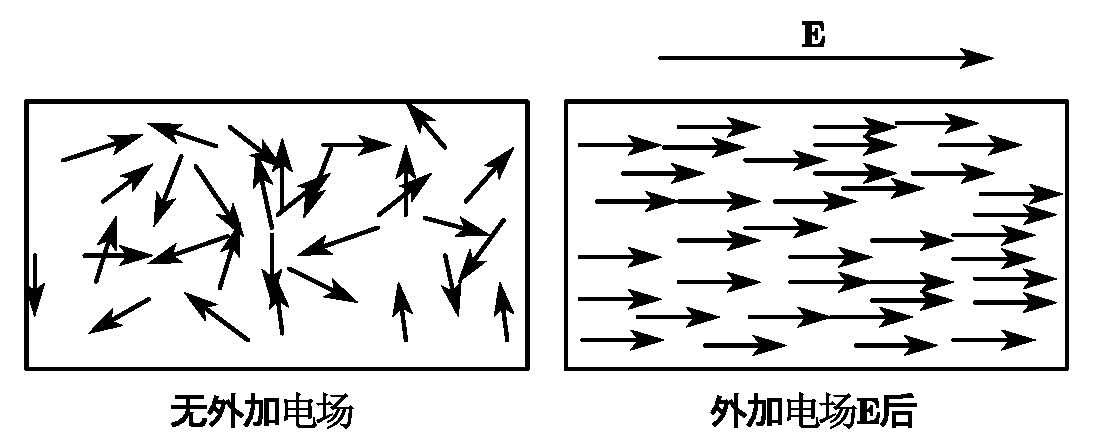
\includegraphics[width=10cm]{./figures/Tensor_1.pdf}
\caption{电场引起电偶极矩变化的示意图.左图中物质里的电偶极子方向随机均匀分布,整体上不显电性;右图中物质里分布着水平向右的电场,在电场作用下电偶极子们都指向水平向右了,出现了水平向右的电偶极矩密度,宏观上开始表现出电性.} \label{Tensor_fig1}
\end{figure}


电偶极矩密度不为零的时候,物质里会出现束缚电荷,但这不是我们目前关心的.我们目前关心的是,电偶极矩密度是怎么被电场影响的.

对于可以自由运动的电偶极子,比如水分子,这个规律其实非常简单:记$\bvec{P}$是某一点的电偶极矩密度,$\bvec{E}$是物质内的电场分布,那么就有$\bvec{P}=\epsilon\bvec{E}$,其中$\epsilon$是一个实数.也就是说,$\bvec{P}$总是和$\bvec{E}$平行,并且大小之比恒为$\epsilon$.这个时候,我们可以说水具有电极化张量$\bvec{M}$,使得$\bvec{P}=\bvec{M}\bvec{E}$.如果按照国际单位制,把$\bvec{E}$和$\bvec{P}$的基都选为同一组直角坐标系上的单位向量,那么水的电极化张量就可以表示为
\begin{equation}
\pmat{\epsilon&0&0\\ 0&\epsilon&0\\ 0&0&\epsilon}
\end{equation}
这是\textbf{单位矩阵的$\epsilon$倍}.

但是电极化张量并非总是这么简单的.如果在一个晶体里,固有的电偶极子都是指向水平方向的,但是水平向右和向左的电偶极子互相抵消,总体上还是不显电性;同时,这些电偶极子无论如何都被限制在水平方向上,那么它们就无法转向.当晶体中存在水平向右的电场$\bvec{E}$的时候,水平向右的电偶极子被拉长、向左的被缩短,于是出现了水平向右的电偶极矩密度$\bvec{P}=\epsilon\bvec{E}$.如果晶体中的电场不在水平方向,那么由于电偶极矩密度还是限制在了水平方向上,因此电场和电偶极矩密度不再平行了.按照国际单位制,把$\bvec{E}$和$\bvec{P}$的基都选为同一组直角坐标系上的单位向量,那么这个晶体里的电极化张量就变成了
\begin{equation}
\pmat{\epsilon&0&0\\ 0&0&0\\ 0&0&0}
\end{equation}
它\textbf{不再是单位矩阵的$\epsilon$倍}.

实际情况下,由于晶格对晶体中电荷在不同方向上的运动有不同程度的阻碍,晶体里的电极化张量不一定是单位矩阵的单位矩阵的倍数.不过,由于改变基时矩阵变为相似矩阵,那么如果电极化张量在某个基下的矩阵表示是可对角化的,那么总能找到$\bvec{E}$的一组基,使得电极化张量的矩阵是一个对角矩阵;换句话说,沿着这基向量方向上的电场,引起的电偶极矩密度依然和电场平行,只不过不同的方向上倍数不一样.

\end{example}


\subsection{$k$阶张量}

\subsubsection{$k$-线性函数}

把$2$-线性函数的定义推广,就得到$k$-线性函数的定义.

\begin{exercise}{}
请尝试给出$k$-线性函数的定义.答案就在题目下方.
\end{exercise}

\begin{definition}{$k$-线性函数}

给定域$\mathbb{R}$上的$n$维线性空间$V$,称$f:V^k\rightarrow \mathbb{R}$为$V$到域$\mathbb{R}$上的一个\textbf{$k$-线性函数},如果$f$对于每一个自变量都是线性的;或者说,当$k$个自变量中只有一个在变化,其它分量不变,那么$f$对于那个变化的自变量是线性函数.特别地,线性函数又被称为$1$-线性函数.

\end{definition}

有了$k$-线性函数的概念,我们就可以定义$k$-阶张量了:

\begin{definition}{张量}
一个$k$-线性函数,被称为一个$k$-阶张量.
\end{definition}

从前面的讨论我们知道,一个二阶张量还可以看成是把一个向量映射到一个向量;向量可以和一阶张量一一对应,因此二阶张量也可以看成是把一个一阶张量映射到一个一阶张量.同样地,一个三阶张量可以看成是把两个线性函数映射到一个一阶张量.

事实上,一个$k$-阶张量$f(\bvec{v}_1, \bvec{v}_2, \cdots,\bvec{v}_k)$是$k$-线性函数,固定住其中几个自变量,比如说$\bvec{v}_1$到$\bvec{v}_m$,那么$f(\bvec{v}_1, \bvec{v}_2,\cdots,\bvec{v}_k)$可以看成是剩下$(k-m)$个自变量的$k-m$-线性函数$g(\bvec{v}_{m+1}, \cdots,\bvec{v}_k)$.也就是说,$f$把前$m$个向量映射成一个$k-m$线性函数.因此,我们也可以说,一个$k$阶张量把$m$个向量映射为一个$(k-m)$-线性函数.

\subsection{小结与拓展}

一个$n$维的$k$阶张量,可以表示为一个$k$维的超立方体矩阵,其中每条边包含了$n$个实数.

我们在之前的定义中都把线性空间看成是定义在实数域$\mathbb{R}$上的,而线性函数是线性空间映射到实数.实际上,这一点可以推广到,把线性空间定义在任何域$\mathbb{F}$上,线性函数就是线性空间映射到这个域$\mathbb{F}$上.这样也可以讨论线性空间上的张量.

目前物理学中常用到的域,是实数域$\mathbb{R}$和复数域$\mathbb{C}$.

像转动惯量这样的物理量,为什么可以看成线性映射呢?这是因为物理量彼此不是独立存在的,多个物理量之间相互作用而影响了其它的物理量,本身就是一种多个物理量映射到其它物理量或它们的性质的过程,就像牛顿第二定律可以看成是把加速度映射到力上,而质量的作用就是作为映射的函数.因此,物理量本身也可以看成是映射的过程,而在许多物理理论中,我们都可以线性地描述这些映射关系,因此常常可以把物理量看成是线性映射.
